%%%%%%%%%%%%%%%%%%%%%%%%%%%%%%%%%%%%%%%%%
% Short Three-Column Newsletter
% LaTeX Template
% Version 1.0 (11/9/13)
%
% Original author:
% Frits Wenneker (http://www.howtotex.com) 
% With extensive modifications by:
% Vel (vel@latextemplates.com)
% 
% This template has been downloaded from:
% http://www.LaTeXTemplates.com
%
% License:
% CC BY-NC-SA 3.0 (http://creativecommons.org/licenses/by-nc-sa/3.0/)
%
%%%%%%%%%%%%%%%%%%%%%%%%%%%%%%%%%%%%%%%%%

%----------------------------------------------------------------------------------------
%	PACKAGES AND DOCUMENT CONFIGURATIONS
%----------------------------------------------------------------------------------------

\documentclass[10pt,a4paper,ngerman,twoside]{article} % Paper type (a4paper, usletter or legal) and font size (10, 11 or 12)

%\setlength\topmargin{-80mm} % Top margin
\setlength\topmargin{-48pt} % Top margin
\setlength\headheight{0pt} % Header height
\setlength\textwidth{7.0in} % Text width
\setlength\textheight{9.5in} % Text height
\setlength\oddsidemargin{-30pt} % Left margin
\setlength\evensidemargin{-30pt} % Left margin (even pages) - only relevant with 'twoside' article option
%\setlength\inner{4cm}
%\setlenfth\outer{2cm}
%\usepackage{geometry}
%\geometry{bindingoffset=20mm}
%\setlength\bindingoffset{2cm}

\usepackage{charter} % Charter font for main content

\frenchspacing % Reduces space after periods to make text more compact for a three-column layout
\usepackage{babel}
\usepackage[utf8]{inputenc}
\usepackage{graphicx} % Required for including images
\usepackage{amssymb} % Math packages
\usepackage{amsmath} 
\usepackage{multicol} % Required for the three-column layout of the document
\usepackage{url} % Clickable links
\usepackage{enumitem} % Reduces the amount of space within and between lists with [noitemsep,nolistsep]
\usepackage{marvosym} % Required for the use of symbols
\usepackage{wrapfig} % Allows wrapping text around figures
%\usepackage[T1]{fontenc} % Use 8-bit encoding that has 256 glyphs
\usepackage{datetime} % Required for defining a custom date style
\newdateformat{mydate}{\monthname[\THEMONTH] \THEYEAR} % Set a custom date format
\usepackage[pdfpagemode=FullScreen, colorlinks=false]{hyperref} % Link colors and PDF behavior in Acrobat
\usepackage{fancyhdr} % Required to define custom headers/footers
\usepackage{hyperref} % funktioniert nicht ?
\pagestyle{fancy} % Enables the custom headers/footers for all pages following this

%-----------------------------------------------------------
% Header and footer
\lfoot{\footnotesize % Left footer containing newsletter contact information
%\begin{wrapfigure}{l}{2.0cm}
%
\includegraphics[width=2cm]{ccbysa88x31.png} 
%\end{wrapfigure}
R.I.S. Journal Ausgabe 001, Jänner 2014: \textbf{R}emix, \textbf{I}mprove, \textbf{S}hare. Das freie, creativ-commons lizensierte Journal.  \\
\Mundus\ Download und andere Formate: \href{http://spielend-programmieren.at/de:ris:start}{\texttt{spielend-programmieren.at/de:ris:start}} \quad
%\Telefon\ (000) 111-1111 \quad
\Letter\ \href{mailto:horst.jens@spielend-programmieren.at}{horst.jens@spielend-programmieren.at}
}

\cfoot{} % Empty center footer

\rfoot{\footnotesize ~\\ Seite \thepage} % Right footer - page counter

\renewcommand{\headrulewidth}{0.0pt} % No horizontal rule for the header
\renewcommand{\footrulewidth}{0.4pt} % Horizontal rule separating the footer from the document
%-----------------------------------------------------------

%-----------------------------------------------------------
% Define separators
\newcommand{\HorRule}[1]{\noindent\rule{\linewidth}{#1}} % Creates a horizontal rule
\newcommand{\SepRule}{\noindent	% Creates a shorter separator rule
\begin{center}
\rule{250pt}{1pt} % Page width and rule width
\end{center}
}
\newcommand{\Trenner}{\noindent
\begin{center}
\rule{100pt}{1pt}
\end{center}
}
%-----------------------------------------------------------

%-----------------------------------------------------------
% Define title and article styles
\newcommand{\NewsletterName}[1]{ % Newsletter title
\begin{center}
\Huge \usefont{T1}{fvs}{b}{n} % Use the Bera Sans Bold font
#1
\end{center}	
\par \normalsize \normalfont}

\newcommand{\JournalIssue}[1]{ % Date and issue number at the top of the newsletter
%\hfill \textsc{\mydate \today, No #1} % Right-aligned date and issue number
\hfill \textsc{Jänner 2014, Ausgabe 001}
\par \normalsize \normalfont}

\newcommand{\NewsItem}[1]{ % News item title
\usefont{T1}{fvs}{n}{n} % Use the Bera Sans Normal font
\vspace{24pt}\large #1\vspace{3pt} % Print the title with space around it in a larger font size
\par \normalsize \normalfont}

\newcommand{\NewsAuthor}[1]{ % Author name under the item title
\hfill von \textsc{#1} \vspace{20pt} % Right-aligned author name in small caps with space after it
\par \normalfont}		

%----------------------------------------------------------------------------------------
%	TITLE
%----------------------------------------------------------------------------------------

\begin{document}

\JournalIssue{1} % Issue number
\NewsletterName{R.I.S. Journal} % Newsletter title
%\begin{center}
%\textbf{R}emix \textbf{I}mprove \textbf{S}hare - das freie Journal für Open Source Education
%\end{center}
\noindent\HorRule{3pt} \\[-0.75\baselineskip] % Thick horizontal rule
\HorRule{1pt} % Thin horizontal rule



%\setlength{\columnsep}{16pt} % Uncomment to manually change the white space between columns
%\begin{multicols}{3} % Begin the three-column layout

%----------------------------------------------------------------------------------------
%	OTHER NEWS
%----------------------------------------------------------------------------------------
%-----------------------------------------------------------
%
%-----------------------------------------------------------
%RIS-Journal Titel (Titelgrafik hier einfügen)
\begin{multicols}{3}
\NewsItem{}
\section*{Die Spieleindustrie ist ein einziger Betrug, arbeite dort nicht!}
\label{redditrant}
\NewsAuthor{gamesindustryvet}

\begin{center}

\includegraphics[width=0.8\linewidth]{redditrant/redditrant-nobody.jpg} \\ % logo ist klein
\footnotesize{anonymer Autor}
\end{center}

\textbf{In diesem \textit{rant} auf der Diskussionsseite \href{http://reddit.com/r/gamedev}{\textit{reddit.com/r/gamedev}} schrieb sich Nutzer 
\glqq
gamesindustryvet
\grqq (Profil mittlerweile gelöscht) 
2012 seinen Frust von der Seele und warnt vor den schlechten Arbeitsbedingungen in der
(U.S. amerikanischen) 
\glqq 
games industry
\grqq 
. \\ Originaltitel: \href{http://www.reddit.com/r/gamedev/comments/z83h2/the_games_industry_is_a_scam_and_this_is_why_you}{\textit{The game industry is a scam and this is why you shouldn't work for it [1]}}} \\

Kommentiert und übersetzt von \href{http://spielend-programmieren.at}{Horst JENS}[2], Abdruck mit freundlicher Genehmigung von \href{http://reddit.com}{\textbf{reddit.com}} \\

(Beginn der Übersetzung)

\subsection*{Posting auf r/gamedev}
Hallo Leute,
ich bin seit 10 Jahren ein Veteran der (Computer)Spieleindustrie. Ich kann es selbst nicht glauben dass ich schon so lange drin bin. Durch anstrengende Misserfolge, gefolgt von noch mehr Misserfolgen (meist das Resultat haarsträubender Management Entscheidungen) hat sich jeder Hauch von Interesse zerstört den ich für diese Branche je hatte.

Ich suche nach Arbeit außerhalb der Branche Dank der in der Computerspieleindustrie gemachten traumatisierenden Erfahrungen. Ein paar Beispiele:

1) Ich arbeitete nonstop 52 Stunden. Ich hatte fast 2 Stunden Schlaf in dieser \textbf{Crunch-time} aber blieb die ganze Zeit über im Büro um das Projekt am Laufen zu halten.   
Weil ich Angststörungen (anxiety disorder) habe nahm ich meine Medikamente nicht (während der Crunch-time) und hatte eienen totalen Zusammenbruch (mental breakdown) am Ende.

2) Ich wurde zwei mal in eine andere Stadt versetzt von einer großen Firma und 3 mal gekündigt (von der selben Firma), jedes mal nicht einmal ein Jahr nachdem ich angefangen hatte. Beim letzten Mal 2 Wochen nachdem ich angefangen hatte.

3) Ich verlor mein Haus, musste Privatkonkurs anmelden (had to file bankruptcy) und humpelte durchs Leben nach meinem ersten Umzug. Ich verlor (die Beziehung zu) vielen Freunde und Verwandten während dieser Zeit wegen Stress.

4) Vor Kurzem arbeitete ich für ein kleines Entwicklungsstudio und musste mich operieren lassen was 2 Wochen Arbeitsausfall nach sich zog. Am Tag nach der Operation wurde ich gekündigt, obwohl mir vorher gesagt wurde es wäre kein Problem wenn ich die Operation machen lasse. Ich hätte wegen der Operation nie meinen Job riskiert... aber warte, das ist die \textit{Games Industry}, da ist jeder Job ständig gefährdet, außer wenn du ein Programmierer (Coder) bist.

Ich wechselte die letzten 5 Jahre mindestens einmal pro Jahr die Firma. Ich war schon lange nicht mehr bei einem Produkt-Launch (Veröffentlichung eines Spiels) dabei wegen der schlechten Entscheidungen die senior manager machten. Viele der Computerspiele (titles) werden gecancelt unabhängig von der Qualität, weil jemand oben in der Hierachie mit irgendeiner Entscheidung nicht einverstanden ist.

Ich brachte enorme Opfer für diese Industrie. Ich bin fast 40 und habe keine Freundin  (no relationship to speak of). Ich lebe in einer fremden, überteuerten Stadt woch ich -wieder einmal- arbeitslos bin, und meine Lebenslauf schaut aus wie Mist (looks like hell). Ich ging auf eine bekannte technische Universität und machte einen begehrten Abschluss (nicht als Programmierer) aber gab das alles auf um meinem Traum zu folgen. 

Dieser Traum wurde total und vollständig vernichtet von den höheren managern. Jenen die lachen, winken und hier auf \textbf{Reddit} darüber posten wie großartig es ist in der \textit{Games Industry} zu sein. Die sind an ihre Position gelangt weil sie die rücksichtslosesten Leute im Geschäft sind und Karrieren, Familien und Nachbarschaften zerstören. Alles damit sie Stars in der \textit{Games Industry} werden obwohl sie außerhalb der Branche niemand kennt. Ich habe Freunde und Kollegen die in dieser Branche waren und physikalisch krank geworden sind, emotionale Schäden haben, und absolut niemand kümmert sich darum wie Mitarbeiter in der \textit{Games Industry} behandelt werden will, hey, da gibt's immer 5 Neue hinter Dir die mehr als willig sind alles zu opfern für den Erfolg der Leute an der Bosse.

Ich hab lange darüber nachgedacht dies alles aufzuschreiben. Ich weiß das viele von Euch (Lesern) in die \textit{Games Industry} rein wollen. Aber ich warne Euch: es gibt einen Grund warum dies ein Erfolgsabhängiges Geschäft ist (hit-driven business), und das alte Herren Netzwerk ist fest eingessesen in dieser Branche. Ich lernte dass hart arbeiten und gute Qualität zu produzieren den Bossen absolut nichts bedeutet. Die wollen dass du das tust. Es wird vorausgesetzt, und wenn du fertig bist mit produzieren schmeissen sie dich raus.

Dieses Geschäft ist ruchlos, halsabschneiderisch und voll mit nachäffenden Firmen (copycat companies) welche versuchen erfolgreichen Titeln die Kunden zu stehlen und  dazu zu bringen den eigenen, unoriginellen Mist zu kaufen. Und hey, mit genug Werbung werden sie auch Erfolg haben.

Die ganze Industrie hat fast gar nichts zu tun mit der Qualität eines Spiel. Ja, manchmal kommen gute Titeln heraus und deren Entwicklungsstudios sind trotz allem erfolgreich. Aber selbst solche Studios (ich denken an das LA Noire team) leiden.

Die \textit{Games Industry} Angestellten verlassen in Scharen diese Branche... nur sagt dir das niemand. Nachdem\textit{ EA-Spouse} unterging war EA's (\textit{Electronic Arts}) Antwort jeden Mitarbeiter unterhalb der Management Ebene nur noch stundenweise zu bezahlen, aber Vollzeitbeschäftigung verlangte mindestens 45 Stunden pro Woche. Wenn du das nicht geschafft hast bekamst du keine Vergünstigungen. Niemand erwähnte das jemals. Zum Glück arbeitete nie wirklich jemand 45 Stunden pro Woche in dieser Branche. Vielleicht tun es diese Executives die man niemals persönlich sieht aber die ihre \textit{Hinter mir die Sinflut} Strategie verfolgen um einen \textit{Hit} zu schaffen. 

Die meisten Angestellten halten es keine 5 Jahre aus. Entweder arbeitest du an einem Titel den du nicht leiden kannst, oder du wirst gefeuert nach dem du dir deine Seele zerstört hast (busting your balls) um einen Titel zu prozieren damit die Spielebranche weiterhin an der harten Arbeit der kleinen Leute profitiert.

Mein Posting wirkt bitter, weil es bitter ist. Meine Karriere ist komplett zerstört, und als Resultat ist mein Ziel Nummer Eins diese Branche zu verlassen. Ich möchte Euch da draußen warnen vor den Risiken wenn man in der \textit{Games Industry} arbeitet.

Ja, es gibt einige wenige (SEHR WENIGE) Entwickler-Studios da draußen die sich um ihre Angestellten ein wenig kümmern aber selbst die großen Namen in diesem business quetschen ihre Leute aus wie Zitronen (run their people into the ground). Und wenn die Leute ganz ausgequetscht sind, dann werden sie ausgespuckt um neuen Trotteln Platz zu machen.

Deine beste Chance, wenn du wirklich mit Computerspielen arbeiten willst, ist es dein eigenes Produkt zu machen. Denk dran, wenn es ein Erfolg wird dann bereite dich darauf vor dass oben erwähnte Spielefiremen tun werden was sie können um deine Idee zu stehlen, und du bist am Ende der Dumme. 

Wenn Computerspiel wirklich das sind was du beruflich machen willst, dann mach es nebenher, zu deinen Bedingungen. Heutzutage ist es einfacher als je zuvor ein eigenes Spiel zu publizieren. Du machst vielleicht nicht das große Geld, du arbeitest vielleicht nicht für ein großes Studio oder einen großen Publisher (glaub mir, das hört sich weit besser an als es ist), aber wenigstens hast du eine professionelle Karriere und wirst (hoffentlich) mit Respekt behandelt und nicht wie eine Ameise unter einer Lupe.\\

EDIT\\

Ich werde nicht auf jedes einzelne posting einzeln antworten aber ich versuche ein paar Fragen zu beantworten. Ich merke dass machen Leute speziell abgestumpft scheinen und ich glaube das sind die Leute die gerade in den Markt eintreten, voll mit Träumen und Hoffnungen wie ich sie damals hatte. Ich glaube ich msus auf die selbe Weise antworten wie schon früher. Ich bin nicht in die Branche reingegangen weil ich mittelmäßig oder faul sein wollte. Ich hatte Leidenschaft, und wer das nicht glaubt ist ein Idiot.

Ich entschuldige mich dafür absichtlich unklar gewesen zu sein, aber ich muss irgendwie meine Gehaltsschecks verdienen. 

1) Mein technischer Uniabschluss war kein Online-Studium.. er war von einer beglaubigten, sehr begehrten Universität. Ich bekam eine akademisches Stipendium, studierte trotz einer Behinderung und arbeitete halbtags um mein Studium zu beenden. Niemand half mir dabei, ich musste alles alleine machen. Ich wuchs sehr arm auf und dass, denke ich, war der einzige Weg um aus diesem Zustand rauszukommen.

2) Meine Situation mag einzigartig für mich sein, aber ich kenne viele Andere deren Erfahrung einzigartig für sie waren, uns die endeten alle mit Burnout. Sie arbeiteten alle sehr hart für einen Traum, während es die Führungskräfte ganz oben unmöglich machten dass dieser Traum in Erfüllung geht.

3) Der Grund warum ich in der 52 Stunden crunch time keine Medikamente nahm war dass ich keine Ahnung hatte dass ich so lange in der Arbeit festsitzen würde. Der Grund war dass ein Manager einen Outsource Entwickler anheuerte der unglaublich Mist baute (screwed us all). Ich hatte keinen Zugriff auf Medikamente. Und lass mich eins klarstellen, ich habe Angststörungen... das macht mich NICHT schwach oder weniger fähig als andere Leute. Ich bin ziemlich sicher ich arbeitete härter als die meisten Leute die ich kenne trotz meiner Behinderung und der Angststörungen (welche über die Jahre schlimmer wurden durch die Schwankungen des Computergame-Marktes).

4) Für ca. 5 Jahre bis zur großen Rezession hatte ich sogar einen milden Erfolg und war konstant bei einer anständigen Firma beschäftigt. Aber das ging zu Ende und ich schaffte es danach für eine sehr lange Zeit nicht durchgehend angestellt zu sein...was es noch schwieriger macht in dieser Industrie wieder Fuß zu fassen. Hier gilt dass du ein Versager bist wenn du nicht an erfolgreichen Titeln beteiligt warst.

5) Ich habe einige meiner Erfahrungen gar nicht aufgeschrieben, hauptsächlich weil sie sehr schmerzhaft für mich waren. Aber ich gewann einige Freunde in dieser Industrie und das Schlimmste ist das durch die ständigen Kündigungen dieses Freunde über die ganze Welt verstreutwerden. Das erlaubt ein brauchbarers virtual network, aber es ersetzt nicht ein Netzwerk von echten Freunden die dich wirklich unterstützen. Wenn du so ein Freundesnetzwerk finden kannst, trotz all der Kündigungen, dann empfehle ich dir dringend dass Du diese Freundschaften ausbaust und pflegst. 

6) Ich bin nicht hierher (\textbf{Reddit}) gegangen um ein allwissender Veteran zu sein oder so etwas. Ehrlich, ich kam her um meine Geschichte zu ezählen, zu erzählen dass ich von vielen anderen ähnlich Schauerhaftes hören musste, und das die Erfolgreichen in dieser Branche die Techniker und die rücksichtslosesten Haie im Geschäft sind. Jede Industrie braucht mehr als nur Programmierer und höhere Manager. Es gibt Designer, Manager, Verwaltungsleute etc. etc.... nur weil jemand kein Programmierer ist macht ihn das nicht wertlos.
 
7) zur 45 Stunden Woche: Das passierte kurz nachdem ich zu Electronic Arts ging. Ich machte diese Erfahrung nicht selbst, sondern einer meiner Mitarbeiter. Ich denke es hörte recht schnell auf sobald die Leute merkten wie illegal es war. Ich denke es dauerte vielleicht ein paar Monate, aber der Punkt ist dass keine dieser Firmen es notwendig finden die Arbeitszeitregelen einzuhalten (none of those companies bother to follow). Ich selbst arbeitete niemals weniger als 45 Stunden pro Woche und ich arbeite sehr sehr hart. 

Wie auch immer, lest aus meinem Posting heraus was ihr wollt. Manche Leute haben Glück in diesem hit-driven business, sehr sehr viele haben kein Glück. Ich wünschte ich hätte solch tolle Erfahrungen gehabt wie sie hier auf \textbf{Reddit} gepostet werden aber das ist mir nie passiert. \\

(Ende der Übersetzung) \\

Das Posting löste eine Reihe von Antworten aus, die man auf \href{http://www.reddit.com/r/gamedev/comments/z83h2/the_games_industry_is_a_scam_and_this_is_why_you}{goo.gl/ivfVkJ}{Reddit.com}[1] direkt unter dem Original-Posting nachlesen und bewerten kann. Neben Ablehnung gab es auch Zustimmung.

\subsection*{Anmerkungen von Horst JENS:}
\begin{center}
\includegraphics[width=0.6\linewidth]{redditrant/horst2011mitdoppeltux.jpg} \\
\footnotesize{Horst JENS. Bildrechte: [2] \href{http://creativecommons.org/licenses/by-sa/4.0/deed.de}{cc-by-sa}}
\end{center}

Als Anbieter von \href{http://spielend-programmieren.at}{Programmierkursen für Jugendliche}[2] und Übersetzer des Postings möchte ich einige Anmerkungen beisteuern:

\begin{itemize}
\item Die Situation des Autors ist wegen der -für europäische Verhältnisse schlechten- U.S. Sozialversicherung nicht Eins zu Eins mit der Situation in Österreich vergleichbar. 
\item Nicht nur wer in der Spielebranche arbeiten will, einfach jeder sollte heutzutage programmieren (coden) können ! Mit moderner Lernsoftware wie z.B. \href{http://scratch.mit.edu}{\textit{Scratch [3]}} ist das in kürzester Zeit möglich, z.B. innerhalb der (kostenlosen) Probestunde bei \href{http://spielend-programmieren.at}{\textit{spielend-programmieren [2]}}! 
\item Ein guter Einstieg in die Spiele-Industrie ist es sicher, ein eigenes (Spiele)Projekt herzeigen zu können bzw. an einem großen (freien) Projekt mitgewirkt zu haben. Zum Beispiel eines der vielen Open Source Projekte auf \href{http://github.com}{Github.com} oder ähnlichen Plattformen. Wer noch nicht so gut programmieren kann findet genügend Aufgaben um sich bei bestehenden Projekten einzubringen, z.B. als Übersetzer, Grafiker, Level-Designer, Bug-Reporter, Tester etc. 
\item Eine andere gute Idee für jeden Interessierten ist es an einem \textbf{GameJam} mitzumachen.  Wer sich beim \href{http://spielend-programmieren.at/de:mailinglist}{\textit{spielend-programmieren Newsletter [3]}} anmeldet wird  über entsprechende Veranstaltungen im Raum Wien per Email informiert.
\item Ich kann den im Posting erwähnten Tipp ('...mach es nebenher, zu deinen Bedingungen...') nur bekräftigen. Ähnlich wie das Spielen eines Musikinstruments hat (Spiele)-Programmierung viel mit Kunst zu tun. Es gibt Künstler, die mit ihrer Musik genug Geld verdienen, aber Geld verdienen sollte nicht der einzige Beweggrund sein ein Musikinstrument zu lernen. Spiele programmieren zu können ist eine Fähigkeit die unter Umständen zu einem Neben- oder gar Hauptberuf werden kann, so wie jedes Hobby. Es ist vor allem eine Fähigkeit mir der man sich selbst und anderen viel Freude machen kann. 
\end{itemize}


\subsection*{Fachbegriffe}

~~~\href{http://reddit.com}{\textbf{Reddit.com}} ist eine größtenteils englischsprachige, sehr beliebte Website welche zu zahlreichen Themen Diskussionsseiten (Webforen) anbietet, sogenannte Sub-Reddits. Im Gegensatz zu simplen Social-Media Seiten wie Facebook oder Google+ sind auf Reddit \textit{Threads} möglich bei Kommentaren, außerdem können einzelne Beiträge und Kommentare sowohl hinauf- als auch hinuterge"voted" werden. Aufgrund des in beide Richtungen möglichen Voting-Mechanismus \textit{schwimmen} beliebte Themen innerhalb einer Gruppe schnell nach oben und bekommen mehr Aufmerksamkeit. Die Registrierung auf Reddit ist kostenlos, und jeder User kann sowohl offene als uach private Subreddits anlegen. Reddit basiert auf \href{http://github.com/reddit/}{\textit{freier Software [5]}}.

\textbf{Crunch-time} (englisch, to crunch: zerbeissen, zermalmen) Zeit kurz vor der Veröffentlichung eines Spieles die von großem Streß gekennzeichnet ist und von den Programmierern Überstunden erfordert, da der Veröffentlichungstermin feststeht und letzte Fehler beseitigt werden müssen.\\

\href{http://de.wikipedia.org/wiki/Thread_(Internet)}{\textbf{Thread}} wörtlich übersetzt Gesprächsleitfaden ist ein Feature von guten Email-Programmen, Usenet-Readern oder Webforen. Es bedeutet dass die einzelnen Nachrichten (bzw. Kommentare oder Emails) nicht streng chronologisch geordnet sind sondern dass eine Antwort B auf eine Nachricht A direkt (und meist nach rechts eingerückt) unter der Nachricht A steht. Siehe auch dieses Schaubild:
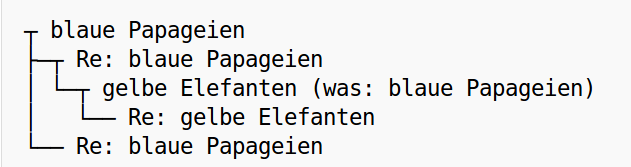
\includegraphics[width=\linewidth]{redditrant/redditrant-threads.png} \\
\begin{center}
\footnotesize{Thread-Darstellung}
\end{center}

\href{https://en.wikipedia.org/wiki/Game_jam}{\textbf{Game Jam}} ist ein organisiertes Treffen bei dem Grafiker, Musiker und Programmierer zusammenkommen um gemeinsam in einer vorgegebenen Zeit (meist ein Wochenende) und zu einem vorgegebenem Thema Computerspiel(e) zu entwickeln. In Österreich wird jährlich im Rahmen des \href{http://globalgamejam.org/}{\textit{Global Game Jam [6]}} der \href{http://austriagamejam.org/}{\textit{Astria Game Jam [7]}} organisiert, zu dem sich jede(r) Interessierte(r) anmelden kann. Andere GameJams werden rein über das Internet organisiert. 
%\begin{center}
%
\includegraphics[width=\linewidth]{redditrant/redditrant-austriagamejam.jpg} \\
%\footnotesize{Austria Game Jam Plakat. Bildrechte: [7]}
%\end{center}


\subsection*{Download, Feedback:}
\footnotesize{
Download: Ordner \texttt{redditrant} \Mundus\ \href{http://spielend-programmieren.at/risjournal/001}{spielend-programmieren.at/risjournal/001}\\
Startseite:\\
\href{http://spielend-programmieren.at/de:ris:001}{spielend-programmieren.at/de:ris:001}\\ 
\Letter\: horst.jens@spielend-programmieren.at\\}
\normalsize 


\subsection*{Lizenz, Quellen:}
\begin{wrapfigure}{l}{2.0cm}

\includegraphics[width=2cm]{redditrant/ccbysa88x31.png} 
%\includegraphics[width=2cm]{horst2011mitdoppeltux.jpg}
%\begin{center}
%\footnotesize{Horst JENS}
%\end{center}
\end{wrapfigure}
Dieses Material steht unter der Creative-Commons-Lizenz Namensnennung - Weitergabe unter gleichen Bedingungen 4.0 International. Um eine Kopie dieser Lizenz zu sehen, besuchen Sie \url{http://creativecommons.org/licenses/by-sa/4.0/deed.de}.

\textbf{Quellen:} \\
{[}1{]} \href{http://www.reddit.com/r/gamedev/comments/z83h2/the_games_industry_is_a_scam_and_this_is_why_you}{goo.gl/ivfVkJ} \\
{[}2{]} \href{http://spielend-programmieren.at}{spielend-programmieren.at} \\
{[}3{]} \href{http://scratch.mit.edu/}{scratch.mit.edu} \\
{[}4{]} \href{http://spielend-programmieren.at/de:mailinglist}{goo.gl/wHP0ID} \\
{[}5{]} \href{http://github.com/reddit/}{github.com/reddit} \\
{[}6{]} \href{http://globalgamejam.org/}{globalgamejam.org} \\
{[}7{]} \href{http://austriagamejam.org/}{austriagamejam} 

\end{multicols}
\SepRule
%-----------------------------------------------------------
\end{document}
